\chapter{Tally Reduction Algorithms}
\label{chap:tally-reduction}

Despite the many advances in Monte Carlo methods over the past few decades, an
efficient parallel implementation for large-scale criticality calculations
capable of scaling on modern petascale supercomputers has not been demonstrated
in the literature. There are a number of factors that hinder the parallel
performance of these calculations as discussed in several recent articles
\cite{pnst-brown-2011, net-martin-2012}.

One traditional limitation was in the implementation of the fission bank in
parallel. In a previous study, we developed a new parallel algorithm for banking
fission sites in a criticality calculation \cite{nse-romano-2012}. Following the
development and analysis of the algorithm, it was implemented in a 3D
constructive solid geometry, continuous-energy Monte Carlo code called OpenMC. A
test of the OpenMC code using this algorithm on the Monte Carlo Performance
Benchmark demonstrated weak scaling up to hundreds of thousands of processors
\cite{ane-romano-2013}. However, in that scaling study, no tallies were included
in the runs, and hence the necessary network communication was greatly reduced.

Alongside studies on advanced parallel methods, there has also been an interest
in methods to reduce correlation between fission source iterations. Gelbard and
Prael first proposed a batching methodology that does exactly that
\cite{pne-gelbard-1990}. Batch statistics have now been adopted by the MC21
Monte Carlo code \cite{physor-kelly-2012}. Other contemporary investigations
have looked at overlapping batch means \cite{ane-ueki-2011}. The present work
describes an ancillary benefit of using batch statistics in parallel
calculations.

%%%%%%%%%%%%%%%%%%%%%%%%%%%%%%%%%%%%%%%%%%%%%%%%%%%%%%%%%%%%%%%%%%%%%%%%%%%%%%%%
\section{Theory}

To construct an estimate for the sample mean and its variance for a physical
quantity in a Monte Carlo simulation, the following formulae are generally used:
\begin{align}
  \bar{x} &= \frac{1}{N} \sum_{i=1}^N x_i \\ s^2_{\bar{x}} &= \frac{1}{N-1}
  \left [ \frac{\sum_{i=1}^N x_i^2}{N} - \left ( \frac{\sum_{i=1}^N x_i}{N}
    \right )^2 \right ]
\end{align}
where $x_i$ is a single realization of the random variable, $\bar{x}$ is the
sample mean, $s^2_{\bar{x}}$ is the variance of the sample mean, and $N$ is the
number of realizations\footnote{A single realization may be the accumulated
  score from a single particle history in a fixed-source calculation or from a
  single fission generation in a criticality calculation.}. A few assumptions
have been made in the use of these formulae; it is assumed that $N$ is large
enough for the law of large numbers and the central limit theorem (CLT) to
apply, and it is assumed that the realizations of the random variable are
independent and identically distributed, again to satisfy conditions of the
CLT. However, in a criticality calculation, it can be shown that there is
significant correlation between successive realizations of the tally random
variables due to the method of successive generations. From a physical
perspective, this correlation arises because fission sites will only migrate so
much from one generation to the next since the mean free path of neutrons is
often much smaller than the overall size of the system. To overcome this
correlation, various Monte Carlo codes instead use batch\footnote{Many people
  use the terms ``batch'', ``generation'', and ``cycle'' interchangeably. In
  this paper, the term ``batch'' specifically refers to the grouping of multiple
  realizations and is generally not the same as a ``generation'' or ``cycle'' in
  a criticality calculation.} statistics whereby $M$ successive realizations of
the random variable are grouped into a single estimate of a new random variable:
\begin{equation}
  y_j = \sum_{i=(j-1)M + 1}^{jM} x_i.
\end{equation}
We note that $M$ must be sufficiently large for the central limit theorem to
apply to the distribution of $y_j$, i.e. the batch must be large enough to
sufficiently reduce correlation between successive batches. The sample mean and
its variance for the new random variable are then
\begin{align}
  \bar{y} &= \frac{1}{N'} \sum_{j=1}^{N'} y_j \\ s^2_{\bar{y}} &= \frac{1}{N'-1}
  \left [ \frac{\sum_{j=1}^{N'} y_j^2}{N'} - \left ( \frac{\sum_{j=1}^{N'} y_j}{N'}
    \right )^2 \right ]
\end{align}
where $N' = N/M$. It is obvious by inspection that the sample mean $\bar{x}$ and
$\bar{y}$ will have the same value regardless of the batching
strategy. Furthermore, while the variances will in general be different, it can
be shown that the expected value of the variances $s^2_{\bar{x}}$ and
$s^2_{\bar{y}}$ are the same. The use of batches provides two main benefits:
\begin{enumerate}
  \item If $M$ is large enough, the random variables that result from the
    batching process are guaranteed to be normally distributed as per the
    central limit theorem.
  \item With a large enough batch size, the correlation between successive
    realizations of the tally random variables becomes negligible, thus ensuring
    that the true variance is not underestimated.
\end{enumerate}

Now let us focus our attention on a situation whereby we are performing a Monte
Carlo simulation on $p$ processors with the entire geometry of the problem
replicated on each processor. After each realization, every processor has its
own accumulated score for the tally variable $x_{i,k}$ where $k$ denotes the
$k$-th processor. Traditionally, to obtain the same answer as would be obtained
in a serial calculation, we would need to take the summation of the tallies (in
MPI parlance, ``reduce'' the tallies) across all processors at the end of the
realization, i.e. $x_i = \sum_{k=1}^p x_{i,k}$. This is depicted in
\autoref{fig:history} where scores inside each box are summed into a single
realization.
\begin{figure}[ht]
  \centering
  \def\svgwidth{2in}
  \input{figures/ch4/history.pdf_tex}
  \caption{Summation of tally scores across processors when doing statistics
    based on a single particle history or single generation.}
  \label{fig:history}
\end{figure}
In terms of network communication, we will need to send at a minimum 8 bytes for
each of the $\ell$ tally bins on $p-1$ processors to the master
process\footnote{This is typically done with the Message Passing Interface by
  calling MPI\_REDUCE.}. Thus, the total amount of data that must be
communicated during the simulation is $8\ell N (p-1)$ bytes since the summation
must be done at every realization. For a simulation with large $\ell$ and/or
large $p$, the time to perform this communication can become prohibitive. An
example of such a scenario is the calculation of the global power distribution
in a large reactor model using a cluster or supercomputer, a calculation easily
requiring millions of tally bins, if not more.

Performing statistics over a batch consisting of multiple realizations somewhat
alleviates the communication requirements while providing other aforementioned
benefits. The summation of tally scores for this scenario is depicted in
\autoref{fig:batch}. Since the reduction now need only be performed at the end
of a batch, the data requirement is then $8\ell N' (p-1)$.
\begin{figure}[ht]
  \centering
  \def\svgwidth{2in}
  \input{figures/ch4/batch.pdf_tex}
  \caption{Summation of tally scores across processors when doing statistics
    based on a single batch with $M=4$.}
  \label{fig:batch}
\end{figure}

\begin{figure}[bht]
  \centering
  \def\svgwidth{2in}
  \input{figures/ch4/batch-parallel.pdf_tex}
  \caption{Summation of tally scores across processors when doing statistics
    based on a batch combining realizations from a single processor with $M=4$.}
  \label{fig:batch-parallel}
\end{figure}
Rather than considering the batch to be the accumulation of scores from many
realizations across many processors, there is no reason that one cannot
reproduce\footnote{Most parallel algorithms in Monte Carlo codes are designed
  such that they do not affect the results of a calculation, i.e. a parallel run
  would reproduce the same answer as a serial run.} the same sample mean, within
floating point precision, by considering a batch to be the accumulation of
scores from many realizations on a single processor. This idea is shown in
\autoref{fig:batch-parallel}. Expressed mathematically, our new random variable
is
\begin{equation}
  z_{j,k} = \sum_{i=(j-1)M + 1}^{jM} x_{i,k}.
\end{equation}
The sample mean and its variance for this random variable would then be
\begin{align}
  \bar{z} &= \frac{1}{N'p} \sum_{j=1}^{N'} \sum_{k=1}^p z_{j,k} \\ s^2_{\bar{z}}
  &= \frac{1}{N'p-1} \left [ \frac{\sum_{j=1}^{N'} \sum_{k=1}^p z_{j,k}^2}{N'p}
    - \left ( \frac{\sum_{j=1}^{N'} \sum_{k=1}^p z_{j,k}}{N'p} \right )^2 \right
  ]
\end{align}
with $N'$ defined the same as before. In this scheme, only one reduction needs
to be performed at the very end of the simulation. The data requirement is then
$16\ell(p-1)$ bytes since we need to take the summation of the accumulated score
and accumulated squares of scores for each tally bin. Thus, the total data that
we need to communicate has been reduced by a factor of
\begin{equation}
  \frac{8\ell N(p-1)}{16\ell (p-1)} = \frac{N}{2}
\end{equation}
For large $N$, as is typical in a Monte Carlo calculation, the reduction in data
communication requirements may significantly improve the parallel efficiency.
  
%%%%%%%%%%%%%%%%%%%%%%%%%%%%%%%%%%%%%%%%%%%%%%%%%%%%%%%%%%%%%%%%%%%%%%%%%%%%%%%%
\section{Results}

To test the efficacy of the proposed method, the ability to perform statistics
based on batches, either across processors or on individual processors, was
implemented in the OpenMC Monte Carlo code. A model of the Monte Carlo
Performance Benchmark \cite{mc-hoogenboom-2011} was then simulated without (Case
1) and with (Case 2) the proposed method on a Linux cluster using eight nodes,
each with two quad-core Intel Xeon E5620 processors for a total of 64 cores. In
both cases, the neutron production rate was tallied over a 289 x 289 x 100 mesh
for a total of 8,352,100 tally bins. Each case was run with 640,000 particles
per generation with 150 inactive batches and 150 active batches\footnote{One
  generation per batch was used for both cases.}. For the neutron cross-sections
and $S(\alpha,\beta)$ tables, ENDF/B-VII.0 data was used. \autoref{tab:time}
shows the elapsed wall-clock times for these two cases.
\begin{table}[bt]
  \centering
  \caption{Elapsed wall-clock time for Monte Carlo Performance Benchmark with
    8,352,100 tally bins.}
  \label{tab:time}
  \begin{tabular}{lcc}
    \toprule
    Variable & Case 1 & Case 2 \\
    \midrule
    Total simulation time     & 1268.7 s & 953.8 s \\
    Time in inactive batches  &  425.3 s & 426.2 s \\
    Time in active batches    &  843.4 s & 527.6 s \\
    Time accumulating tallies &  348.8 s &  30.4 s \\
    \bottomrule
  \end{tabular}
\end{table}
We see that not taking the summation of the tallies across processors at every
generation results in a significant reduction in elapsed time. Most importantly,
the time spent accumulating tallies was reduced by over 90\%. The gross
reduction in simulation time will depend on many factors including simulation
parameters (e.g. how many particles are run per generation) as well as the
specific hardware for the system being used (e.g. network latency and
bandwidth).

\begin{figure}[ht]
  \centering
  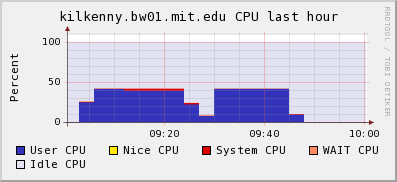
\includegraphics[width=3in]{figures/ch4/cpu_usage.png}
  \caption{Percentage CPU usage of entire cluster during two simulations of the
    Monte Carlo Performance Benchmark.}
  \label{fig:cpu-usage}
\end{figure}
\begin{figure}[ht]
  \centering
  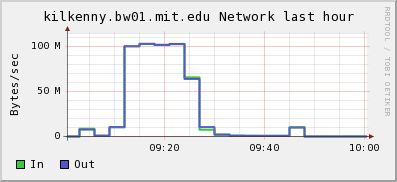
\includegraphics[width=3in]{figures/ch4/network.png}
  \caption{Network bandwidth during two simulations of the Monte Carlo
    Performance Benchmark.}
  \label{fig:network}
\end{figure}
\autoref{fig:cpu-usage} and \autoref{fig:network} show the CPU usage and network
communication, respectively, as reported by the Ganglia Monitoring System. On
\autoref{fig:cpu-usage}, no pause is observed between cases 1 and 2 as they were
run back-to-back. The case 2 run began at 9:29.

One can see from these figures that during the second simulation, where
reductions on tallies were not performed until the end of the simulation, the
network usage was drastically lower than when reductions were performed at every
generation. Lastly, we remark that all reported sample means of the tally
variables were identical and almost all variances were within two standard
deviations of one another.

%%%%%%%%%%%%%%%%%%%%%%%%%%%%%%%%%%%%%%%%%%%%%%%%%%%%%%%%%%%%%%%%%%%%%%%%%%%%%%%%
\section{Discussion}

A novel scheme for reducing data communication requirements in parallel Monte
Carlo calculations has been introduced here primarily aimed at criticality
calculations. In a large-scale simulation with thousands of processors, it is
natural to consider the batch to be the accumulation of scores from one
processor over the entire run ($M = N$). Provided each processor did a
sufficient amount of work to obtain reasonable statistics, the estimate of the
variance of the sample mean will be reliable since one would have $p$
realizations of the random variable.

One concern that might arise from the use of this technique is that the variance
of the sample mean will not be reproducible when running in parallel, i.e. the
variance of the sample mean will not be the same as if one had run the exact
same calculation in serial. However, the {\it expected value} of the sample
variance will be the same and the sample mean will be reproduced to within
floating point error. For users who are willing to sacrifice reproducibility of
tally variances, this detriment does not outweigh the overwhelming benefit of
drastically reduced network communication and improved parallel efficiency.

It should be noted that this method does require that the sum and sum of squares
over realizations for each tally bin be stored in memory on each
processor. Strictly speaking, the traditional methods only require storing a
temporary variable on each slave processor to accumulate scores that would be
sent to the master, i.e. the sum and sum of squares for each tally bin need to
be stored only on the master process. However, some, if not many, Monte Carlo
codes do not take advantage of this fact and simply replicate all tally data in
the memory of each process.

As a final note, even when this method is used, it may still be desirable to
perform a reduction over some global tallies such as the eigenvalue. Since the
eigenvalue is used in determining the average number of fission sites produced
at each collision, reproducibility of the sample means of local tallies can only
be preserved if the eigenvalue is the same as it would have been in a serial
run. The parallel communication necessary to perform a parallel reduction of
global tallies such as the eigenvalue will be very small since it is generally
limited to only a few quantities.
